\cleardoublepage


\chapter{Introducción}
\label{ch:chapter1}


\section{Motivación y Objetivos}\label{sec:motivación-y-objetivos}

El área del deep learning ha avanzado exponencialmente en los últimos años.
Esto ha permitido que a día de hoy se pueda contar con modelos predictivos capaces de procesar imágenes y clasificarlas según sus características primarias.
La consecuencia principal de este proceso es la apertura de una ventana de oportunidad a la explotación de estos modelos en un entorno real, con el objetivo de que sean cruciales a
la hora de detectar incendios, terremotos, así como todo tipo de desastres naturales.
El uso eficiente de estos modelos requiere de una infraestructura capaz de soportar la fiabilidad necesaria en términos de robustez y velocidad.
En estos casos, el procesamiento en tiempo real se vuelve algo indispensable para lograr optimizar recursos de emergencia, dirigir equipos a las zonas de desastre más afectadas,
y, en definitiva, prevenir los máximos riesgos posibles.
Los ejes que vertebran este proyecto se sitúan en torno a dos polos: primeramente, la aceleración del tiempo de entrenamiento de un modelo de deep learning usando una gpu en el
servicio de Google Colab, y en segundo lugar, la optimización del tiempo de inferencia del modelo mediante Openvino.
Finalmente, el modelo se desplegará en un entorno cloud en el que pueda funcionar como servicio capaz de sopotar miles de llamadas concurrentes.
La consecución del objetivo general anteriormente mencionado se lleva a cabo en la presente memoria abordando una serie de objetivos específicos, los cuales se enumeran a
continuación:
\begin{itemize}
    \item Mejora en los tiempos de entrenamiento de un modelo de deep learning usando una gpu del servicio de Google Colab.
    \item Conversión de un modelo de tensorflow a uno de Openvino para aumentar la velocidad de inferencia del mismo.
    \item Preparación de una arquitectura de Google cloud capaz de soportar tráfico concurrente en tiempos óptimos para el servicio.
    \item Codificación de una aplicación capaz de hacer uso de los distintos sistemas de inferencia de Tensorflow y Openvino.
    \item Codificación de una aplicación web apta para exponer todos los servicios en un entorno productivo.
    \item Encapsulación de los distintos entornos de producción haciendo uso de Docker.
    \item Despliegue de la aplicación y pruebas de carga.
    \item Obtención de resultados y realización de comparativas de rendimiento entre los distintos sistemas de inferencia, hardware y servidores web.
\end{itemize}


\section{Concepto Deep Learning}\label{sec:concepto-deep-learning}
La inteligencia artificial actualmente se compone de varias ramas tales como machine learning, natural language processing, entre otras.
Una de ellas es el deep learning. Esta arquitectura de aprendizaje profundo persigue el aprendizaje y clasificación de una variedad de problemas
haciendo uso de sus propios algoritmos;
algoritmos que basan su estructura en redes neuronales artificiales, imitando el comportamiento que tienen las del ser humano y su sistema nervioso central.

\subsection{Estado del arte}\label{subsec:estado-del-arte}
En la actualidad, los algoritmos de deep learning son usados para todo tipo de problemas que abarcan multitud de sectores dentro de la industria, los gobiernos, y en definitiva, de la propia sociedad.
La digitalización y expansión de internet provee de innumerables fuentes de datos capaces de ser procesadas y analizadas por este tipo de algoritmos, que son usadas para distintos fines.
Los gobiernos poseen sus sistemas personales de reconocimiento de imágenes para la clasificación de sus ciudadanos, sistemas de recomendación tanto para las empresas que buscan aumentar sus ventas como para bancos que buscan gente apta para préstamos e
incluso sirve como sesgo para evitar contenido indeseable en plataformas a través de la red.
En general, la cantidad masiva de datos ha creado una necesidad de explotación a
través de los mismos , por lo que el deep learning se sitúa como una herramienta fiable para dar valor a todas las interacciones que están ocurriendo casi de manera permanente
en cada sistema tecnológico del planeta.

\subsection{Redes neuronales en el tratamiento de imágenes}\label{subsec:redes-neuronales-en-el-tratamiento-de-imágenes}
La unidad básica de procesamiento de las redes neuronales es el perceptrón, a partir del cual se desarrolla un algoritmo capaz de generar un criterio para seleccionar un sub-grupo a partir de un grupo de componentes más grande.
Este conjunto de neuronas pasará a formar parte de las distintas capas que componen por completo la red neuronal.
Cada neurona recibe una entrada, ya sea de una fuente externa o de otra neurona.

\begin{figure}
    \centering
    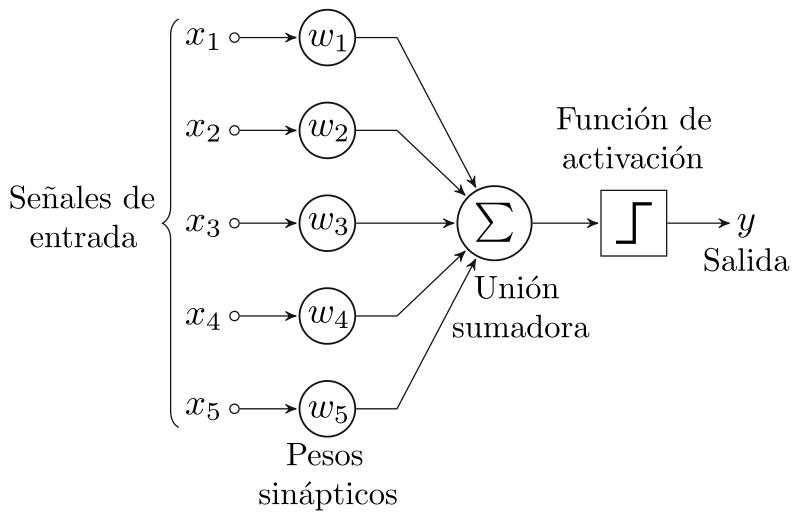
\includegraphics[width=0.6\textwidth]{images/chapter1/perceptron.png}
    \caption{Ejemplo de perceptrón.}
    \label{fig:Perceptrón}
\end{figure}
A partir de aquí cada neurona aplica una función de cálculo a partir de los pesos mediante la cual acaba propagando el resultado a las capas posteriores, y
finalmente a la capa de salida mediante la que podremos obtener nuestra clasificación final.
En este problema concreto, nos centramos en clasificar imágenes multiespectrales,
que consisten en la captura de datos de imágenes dentro de rangos de longitud de onda específicos a través del espectro electromagnético.
Nuestro conjunto de imágenes multiespectrales pertenece a una zona parcialmente destruida por un desastre natural.
El objetivo de nuestro algoritmo de deep learning es tener la capacidad de clasificar dichas imágenes dependiendo si la zona está dañada o,
por el contrario, está en buenas condiciones.


\section{Organización de esta memoria}\label{sec:organización-de-esta-memoria}

Teniendo presentes los anteriores objetivos concretos, se procede a describir la organización del resto de esta memoria, estructurada en una serie de capítulos cuyos contenidos se
describen a continuación:

\begin{itemize}
    \item \textbf{Entrenamiento del modelo mediante Google colab}: Se define el proceso de entrenamiento y aumento de la velocidad del mismo usando la plataforma Google colab
    \item \textbf{Tecnología Openvino}: Se define el propósito de la herramienta de Intel Openvino así como la transformación de un modelo de tensorflow para que sea compatible con openvino.
    \item \textbf{Arquitectura Cloud propuesta}: Se presenta la arquitectura de Google Cloud diseñada para soportar toda la infraestructura de la aplicación y se explica la puesta en producción del servicio.
    \item \textbf{Resultados experimentales}: Se preparan los distintos frameworks web que van a ser puestos a prueba haciendo uso del lenguaje de programación Python.
    \item \textbf{Conclusiones y trabajo futuro}: Se presentan los resultados obtenidos mediante las pruebas de carga y también algunas posibles líneas de trabajo futuro que se pueden desempeñar en relación al presente trabajo.
\end{itemize}